\chapter{Travail réalisé}

Ce chapitre présente le travail réalisé durant le stage. Toutes les tâches relatives au planning
décrit précédemment ont pu être effectuées.

\section{Création de l'environnement virtuel}

Pour la création de l'environnement virtuel, nous nous sommes d'abord tourné vers Anaconda.
Bien que très puissant, cet outil est assez lourd et il est complexe de lister des dépendances
sans préciser les versions, ce qui nous a posé des problèmes de compatibilité entre les différentes
librairies.
Nous avons donc décidé de créer un simple fichier \texttt{requirements.txt} qui liste
toutes les dépendances, et permet de les installer en utilisant la commande
\texttt{pip install -r requirements.txt}.\\

Ce fichier a permis de porter l'environnement de développement sur toutes les machines
à notre disposition, et permettra au prochains développeurs de reprendre le projet.

\section{Documentation initiale}

Étant la seule personne familière avec les techniques de machine learning, j'ai pris soin de documenter
et présenter à l'équipe les différents concept utilisés durant le stage. Cette section présente
les éléments que j'ai abordé.

\subsection{COCO (Common Objects in COntext)}

Le format COCO \cite{Lin_Maire_Belongie_Bourdev_Girshick_Hays_Perona_Ramanan_Zitnick_Dollar_2015}
est un format d'annotation d'images très utilisé dans le domaine de la détection d'objets,
qui a été proposé par Microsoft.
Il est l'un des deux formats acceptés pour l'entraînement de YOLOX, avec le format VOC.
Un dataset COCO est composé d'un dossier comprenant des images, et d'un fichier json qui contient les annotations.
Ce dernier est structuré en quatre parties :
\begin{itemize}
    \item des informations générales sur le dataset (date de création, version, licence, etc.) ;
    \item les catégories d'objets présents dans le dataset ;
    \item les informations sur les images (nom, taille, etc.) ;
    \item les annotations des objets détectés dans les images.
\end{itemize}

Les annotations peuvent contenir un paramètre booléen \texttt{iscrowd} qui indique si
la détection contient plusieurs objets en même temps. Ce paramètres nous a permis d'écarter
ce genre de détection, car notre tâche consiste en la détection de bateaux individuels,
et non d'ensemble de bateaux. \\

En plus d'être un format de dataset, COCO est aussi un dataset en lui-même, disponible
en ligne : \url{https://cocodataset.org/#home}.
Il est composé de plus de 200 000 images annotées pour différentes sortes de tâches d'apprentissage machine.
Parmi toutes ces images se trouvent environ 3000 images de bateaux, qui ont été utilisées
l'année dernière pour entraîner le modèle YOLOX. \\

Lors du téléchargement de ce dataset, nous avons remarqué que la partie test n'était pas annotée.
Ceci est dû au fait qu'elle est destinée à être utilisée pour des compétitions de détection d'objets :
les participants soumettent leurs prédictions sur cette partie, et les résultats sont calculés par les
serveurs de COCO.\\

\subsection{Data augmentation}

Afin d'améliorer la généralisation du modèle, nous avons exploré les différentes méthodes de data augmentation,
et nous avons été chargé de les exposer à l'équipe. Nous nous sommes basés
sur les travaux de \cite{Mumuni_Mumuni_2022}.

\subsubsection{Techniques principales}

Les techniques les plus classiques sont basées sur la géométrie de l'image :
\begin{itemize}
    \item rotation ;
    \item translation ;
    \item recadrage ;
    \item miroir.
\end{itemize}

Il existe aussi des techniques basées sur la modification des couleurs :
\begin{itemize}
    \item luninance ;
    \item saturation ;
    \item contraste ;
    \item teinte.
\end{itemize}

Enfin, il est possible d'ajouter du bruit à l'image, appliquer un flou gaussien ou encore
un flou de bouger.

\subsubsection{Data augmentation dans YOLOX}

La documentation de YOLOX (\url{https://yolox.readthedocs.io/en/latest/}) ne liste pas de manière
exhaustive les techniques de data augmentation intégrées, mais nous avons pu en identifier quelques unes
en étudiant le code source.

Mixup est une technique proposée par Zhang et al. \cite{Zhang_Cisse_Dauphin_Lopez} qui consiste à combiner
deux image en réduisant leur opacité. La mosaïque est une technique qui consiste à
acoller plusieurs images pour en former une seule.

\begin{figure}[H]
    \centering
    \begin{minipage}{.5\textwidth}
      \centering
      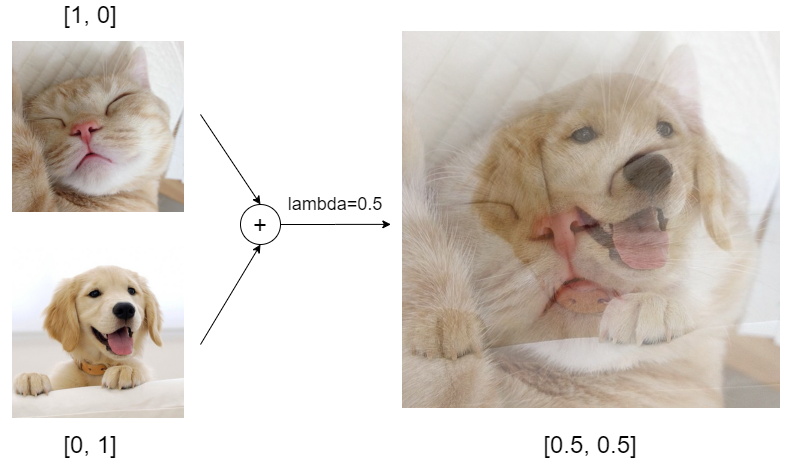
\includegraphics[width=0.6\textwidth]{./img/mixup_augmentation.png}
      \captionof{figure}{Exemple de mixup}
      \label{fig:test1}
    \end{minipage}%
    \begin{minipage}{.5\textwidth}
      \centering
      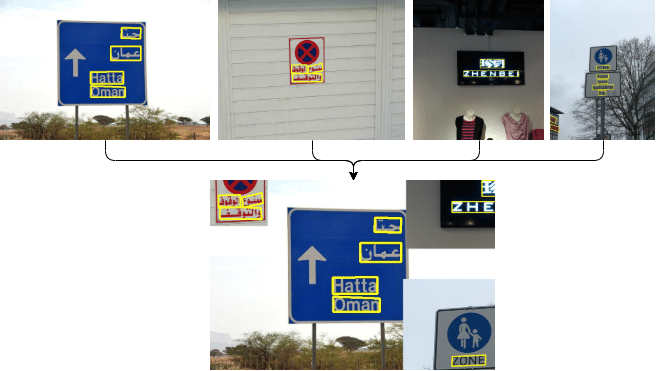
\includegraphics[width=0.6\textwidth]{./img/mosaic_augmentation.png}
      \captionof{figure}{Exemple de mosaïque}
      \label{fig:test2}
    \end{minipage}
\end{figure}

Bien que cette technique ne soit pas explicitement mentionnée dans la documentation,
nous avons pu identifier des transformations de couleurs dans le code source,
ainsi qu'un paramètre associé dans le fichier de configuration.
C'est une technique de modification des couleurs.

Dans le code source, il est possible de spécifier un nombre d'époques sans augmentation.
Nous n'avons pas trouvé de documentation sur cette technique.\\

Après discussion avec l'équipe, il a été décidé que les technique déjà intégrées à YOLOX
couvraient la plupart des augmentations possibles, et qu'il n'était pas nécessaire d'investir
du temps de développement pour en ajouter d'autres. De plus, cela était également déconseillé
par des développeurs ayant déjà travaillé avec YOLOX.\\

\subsection{Métriques d'évaluation d'un modèle de détection}

Afin de mesurer la performance de notre modèle de façon objective,
nous avons utilisé les métriques suivantes :
\begin{itemize}
    \item mAP (mean Average Precision) : moyenne des précisions pour chaque classe ;
    \item mAR (mean Average Recall) : moyenne du rappel pour chaque classe ;
\end{itemize}

Ces métriques sont caclulées de la façon suivante :\\

$$
\text{mAP} = \frac{VP}{VP + FP}
$$

$$
\text{mAP} = \frac{VP}{VP + FN}
$$

avec $VP$ les vrai positifs, $FP$ les faux positifs et $FN$ les faux négatifs (\textit{voir illustration en annexe }
\ref{precision_recall}).\\

Les prédiction du modèle consistent en des boîtes englobantes, qui sont des rectangles délimitant
l'objet détecté. Pour mesurer la précision et le rappel, il faut déterminer si la prédiction
est vraie ou fausse. Pour cela on utilise un seuil IoU (Intersection over Union,
\textit{voir annexe\ref{iou}}) :
\[
    IoU = \frac{A_{\text{intersection}}}{A_{\text{union}}}
\]

Si l'IoU est supérieur à un certain seuil, la prédiction est considérée comme vraie.\\

Dans notre cas, la precision a une grande importance : comment mentionné précédemment,
un faux positif a des conséquences très négatives sur la perception du produit par le client.

Un élément important à noter est que ces deux métriques sont dépendantes : plus la précision est élevée,
plus le rappel est faible, et inversement. Lors de l'inférence du modèle, chaque détection est accompagnée
d'un score de confiance, qui permet de déterminer si la détection est fiable ou non. Appliquer un seuil
sur ce score permet de régler le compromis entre précision et rappel.\\

\section{Datasets}

Après avoir terminé la documentation, nous avons commencé la collecte d'images.
L'entraînement d'un modèle d'apprentissage automatique nécessitant un grand nombre d'exemples,
nous avons consacré plusieurs semaines à la recherches d'images de bateaux annotées.
Le résultat de ces recherches est une combinaison de plusieurs datasets existants :
ABOships-PLUS, boat\_computer\_vision\_project, coco\_boats, dataset\_GLSD, lajolla\_v5,
marvel\_single\_v1, mcships, mods, official\_buoy\_detection, open\_images, open\_images\_lighthouse,
orda, SeaDronesSee, SeaShips, singapore\_maritime, SMD Plus, vais\_old, vessel\_detection\_v21


L'ensemble des données récoltées représente plus de 117 000 images annotées, contenant environ 390 000 bateaux.
Nous avons été vigilant lors de la collecté à n'utiliser que des datasets qui, selon leurs auteurs,
étaient libres de droits (sans pour autant pouvoir le vérifier).
Pour pouvoir comparer nos résultats d'entraînements, nous avons décider de constituer un dataset
de test unique. Nous avons pour cela utilisé 10\% de toutes nos images, et nous avons conservé ce dataset
jusqu'à la fin du stage.

\section{Prise en main des outils}

\subsection{FiftyOne}

FiftyOne est un outil open source permettant de visualiser des datasets, les filtrer,
détecter les doublons, les erreurs de détections et bien d'autres fonctionnalités.
Il a été d'une grande utilité lors de nos travaux, en particulier pour explorer facilement
des datasets conséquents, et montrer les résultats d'inférences
à des collègues non spécialistes.\\

Après avoir récolté des datasets, nous avons entrepris de les importer dans ce logiciel. Cette étape à
nécessité le développement de plusieurs scripts de conversion, car il existe un grand nombre de format
d'annotation pour la détection d'objets. FiftyOne était compatible avec COCO, c'est celui-ci que nous
avons choisi pour travailler tout au long du stage.\\

\subsection{YOLOX}\label{yolox}

\subsubsection{Présentation}

YOLOX est un modèle de détection d'objets en temps réel, basé sur YOLOv5. Il permet de rapidement
localiser et identifier des objets dans une image.

Les réseaux de neurones de la famille YOLO (You Only Look Once) sont composés de trois parties
\cite{Redmon_Farhadi_2018} : head, neck et backbone.
La partie backbone permet d'extraire les features \footnote{Les features sont une représentation des
caractéristiques de l'image sous forme de vecteur.} de l'image, la partie neck est chargée de retrouver les informations spaciales,
et la partie head permet de prédire les boîtes englobantes, les classes et les scores de confiance.\\

Dans leur article, les auteurs de YOLOX \cite{Ge_Liu_Wang_Li_Sun_2021} introduisent une nouvelle méthode
pour améliorer la détection d'objets : la décorrélations entre la classification de l'objet et
sa localisation. Cette méthode a permis d'améliorer significativement les performances du modèle.\\

Ce dernier est disponible en plusieurs versions (\url{https://yolox.readthedocs.io/en/latest/model_zoo.html#standard-models}):
\begin{itemize}
    \item YOLOX-nano ;
    \item YOLOX-tiny ;
    \item YOLOX-S (small) ;
    \item YOLOX-M (medium) ;
    \item YOLOX-L (large) ;
    \item YOLOX-X (extra large) ;
    \item YOLOX-Darknet53.
\end{itemize}

Ces versions correspondent à différents paramètres de largeur et profondeur des couches de neurones.
Ces paramètres sont modifiables directement dans le fichier de configuration,
et on peut observer leur effet sur la structure du modèle grâce à l'outil Netron
(\url{https://netron.app}).

Les modèles les plus légers sont les plus rapides, mais ont une précision plus faible.
L'année précédent, le choix du modèle s'est porté sur YOLOX-S, qui est un bon compromis entre
vitesse et précision.\\

Les poids des modèles sont disponibles en ligne. J'ai été chargé au début du stage de les
télécharger et de les tester une première fois sur des images de bateaux, afin de vérifier
le bon fonctionnement de l'environnement.\\

\subsubsection{Entraînement}

Après avoir exécuté les scripts de démonstration pour tester l'environnement
et fait une première inférence \footnote{L'inférence est le processus de prédiction
de l'objet dans une image.}, nous avons entrepris d'entraîner le modèle sur nos datasets spécialisés pour
les bateaux. Cet étape a été complexe, car certaines fonctions n'était pas documentées, et
la structure du dossier pour le dataset d'entraînement était implicite. Nous avons donc pris soin de documenter
ces informations. Après avoir réussi à entraîné le modèle, nous avons activé l'outil
Weight and Biases (\url{https://wandb.ai/home}) pour suivre l'évolution de l'entraînement.\\

Pour vérifier la cohérence des résultats, nous avons effectué trois entraînements avec 3000, 5000
et 10000 images. Nous nous attendons à une augmentation de la précision avec l'augmentation du dataset,
ce qui était le cas :

\begin{figure}[H]
    \centering
    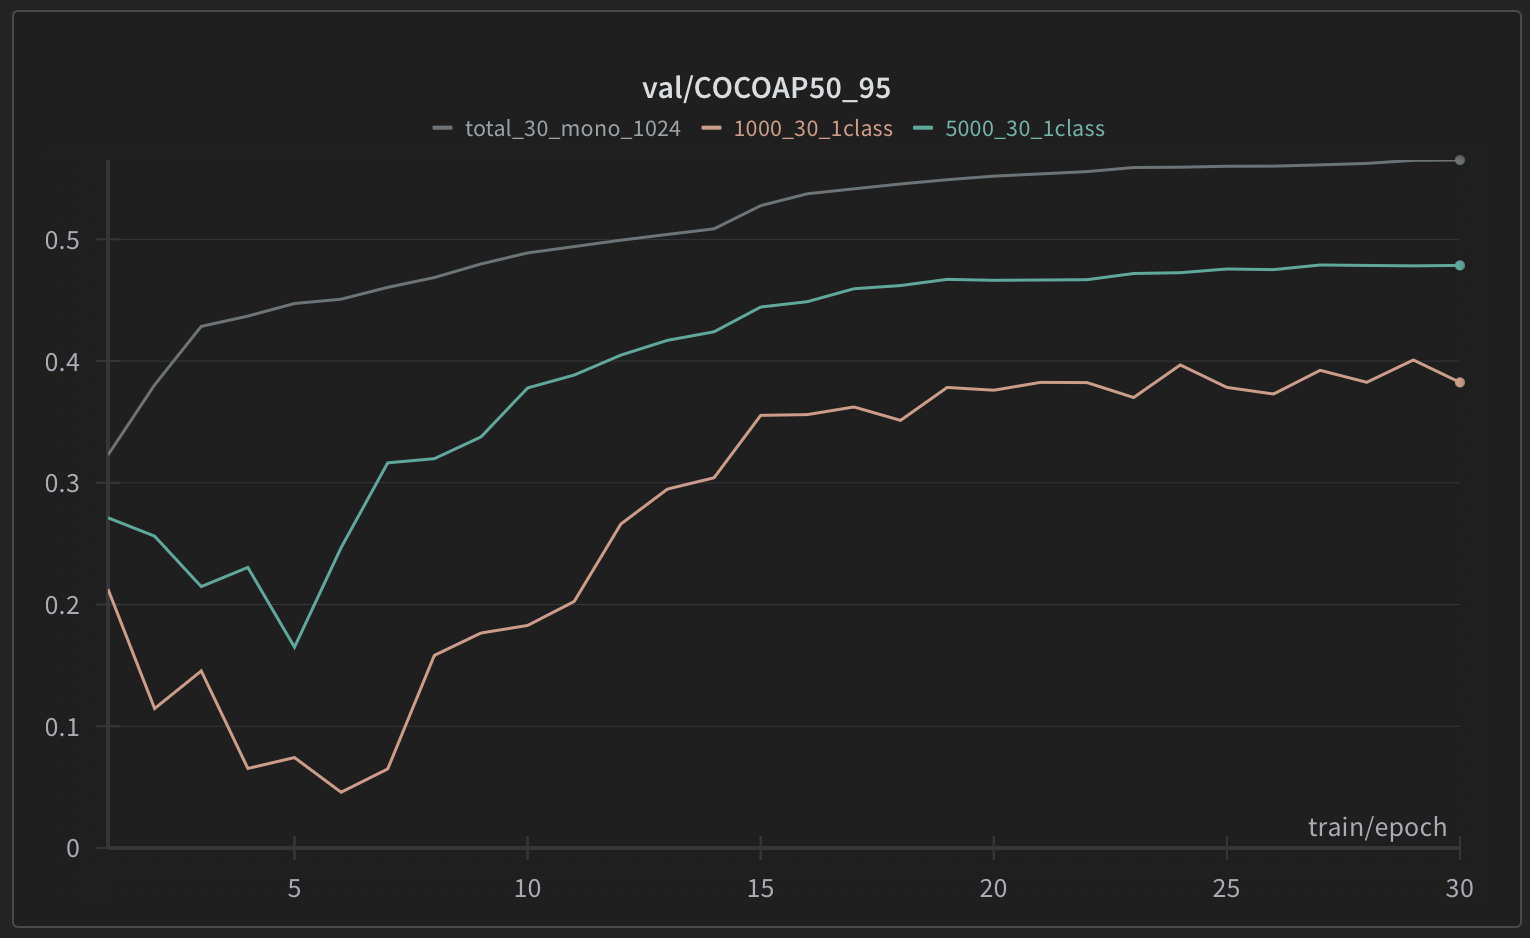
\includegraphics[width=0.5\textwidth]{./img/dataset_size.png}
    \caption{Évolution de la précision en fonction de la taille du dataset}
\end{figure}

Cet expérimentation nous a également donné l'opportunité d'analyser la courbe de précision sur le dataset
de validation : on peut distinguer une baisse de mAP pendant les cinq première époques appelée "warmup",
et une augmentation de la précision 15 époques avant la fin, qui correspond à l'arrêt de la data augmentation.\\

\subsubsection{Évaluation}

Pour obtenir des score représentatifs de la performance du modèle, nous avons évalué YOLOX
sur le dataset de test. Il est nécessaire d'ajouter le paramètre \texttt{--test} à la commande
d'évaluation, sinon le modèle est évalué sur le dataset de validation (ce qui n'était pas mentionné
dans la documentation). Voici le résultat d'une évaluation du modèle :

\begin{verbatim}
    Average forward time: 27.18 ms, Average NMS time: 2.22 ms, Average inference time: 29.41 ms
    Average Precision  (AP) @[ IoU=0.50:0.95 | area=   all | maxDets=100 ] = 0.699
    Average Precision  (AP) @[ IoU=0.50      | area=   all | maxDets=100 ] = 0.945
    Average Precision  (AP) @[ IoU=0.75      | area=   all | maxDets=100 ] = 0.766
    Average Precision  (AP) @[ IoU=0.50:0.95 | area= small | maxDets=100 ] = 0.396
    Average Precision  (AP) @[ IoU=0.50:0.95 | area=medium | maxDets=100 ] = 0.623
    Average Precision  (AP) @[ IoU=0.50:0.95 | area= large | maxDets=100 ] = 0.832
    Average Recall     (AR) @[ IoU=0.50:0.95 | area=   all | maxDets=  1 ] = 0.331
    Average Recall     (AR) @[ IoU=0.50:0.95 | area=   all | maxDets= 10 ] = 0.713
    Average Recall     (AR) @[ IoU=0.50:0.95 | area=   all | maxDets=100 ] = 0.736
    Average Recall     (AR) @[ IoU=0.50:0.95 | area= small | maxDets=100 ] = 0.501
    Average Recall     (AR) @[ IoU=0.50:0.95 | area=medium | maxDets=100 ] = 0.680
    Average Recall     (AR) @[ IoU=0.50:0.95 | area= large | maxDets=100 ] = 0.858
    per class AP:
    | class   | AP     |
    |:--------|:-------|
    | boat    | 69.932 |
    per class AR:
    | class   | AR     |
    |:--------|:-------|
    | boat    | 73.551 |

\end{verbatim}

On retrouve les métriques mAP et mAR, avec différents seuils d'IoU, et pour différentes tailles d'objets :

\begin{itemize}
    \item small : area < 322 pixels ;
    \item medium : 322 < area < 962 pixels ;
    \item large : area > 962.
\end{itemize}

Naturellement, les scores sont générallement plus faibles lorsque les objets sont petits.

\subsubsection{Inférence}

Pour terminer la vérification de notre environnement, nous avons écrit des scripts permettant de
transférer les résultats des inférences de nos modèles entraînés dans FiftyOne, afin de mieux visualiser
nos résultats. Voici une comparaison entre un des premiers modèles que nous avons entraîné, avec 30 000 images
de navires, et d'autres modèles classiques :

\begin{figure}[H]
        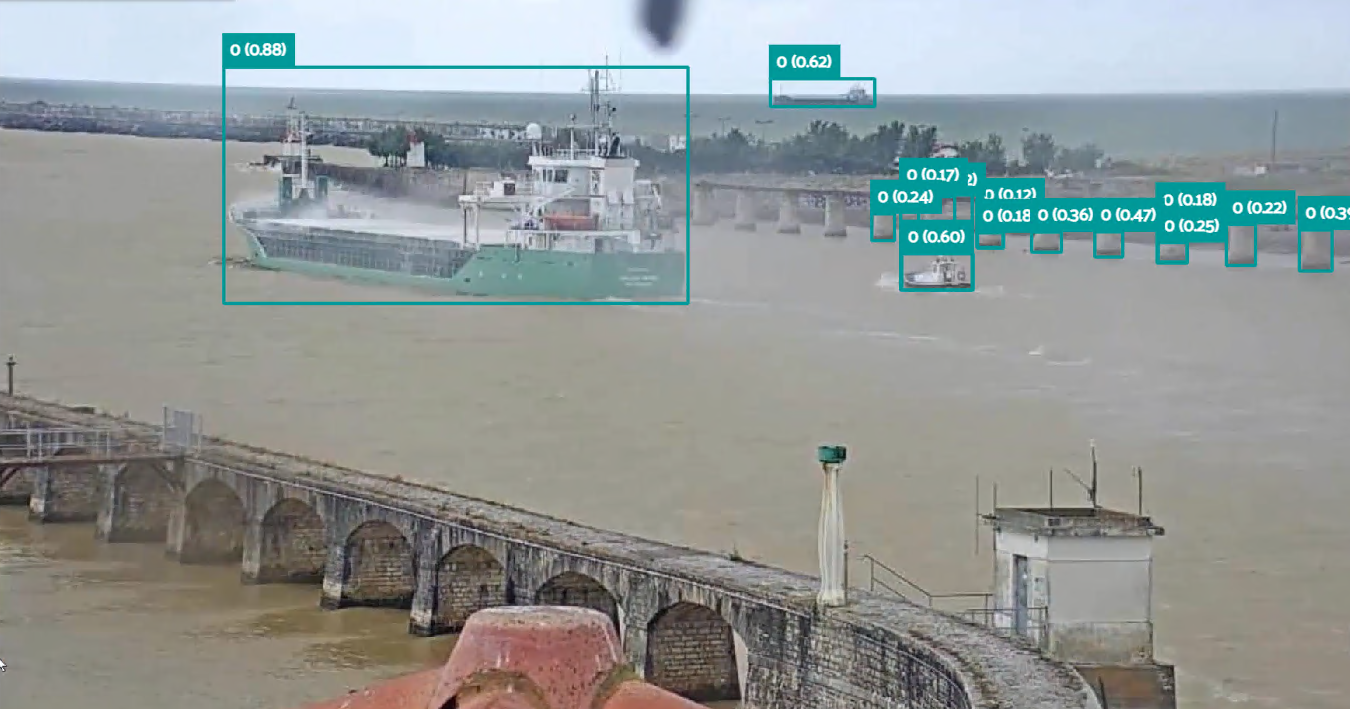
\includegraphics[width=0.5\textwidth]{./img/first_inference.png}
        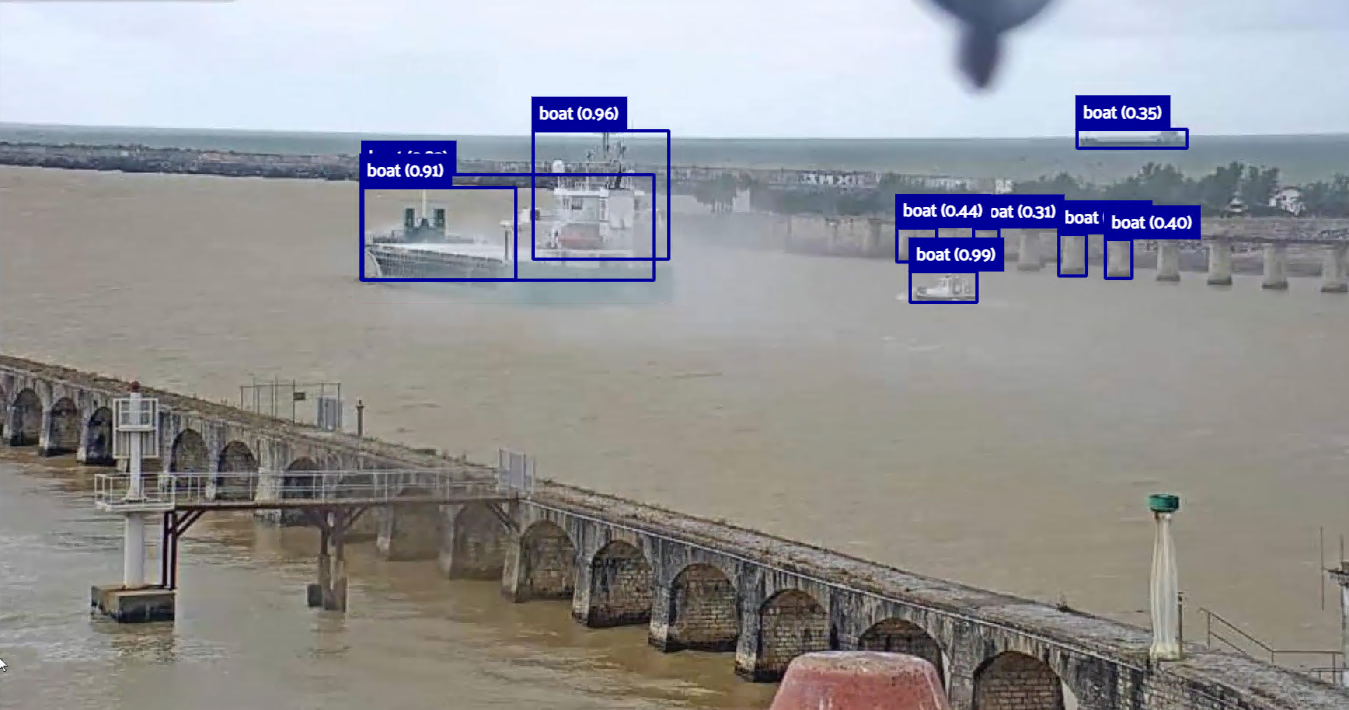
\includegraphics[width=0.5\textwidth]{./img/resnet_inference.png}
        \caption{Comparaison entre notre premier modèle entraîné (\textit{à gauche}) et ResNet50 (\textit{à droite}).}
\end{figure}

\begin{figure}[H]
    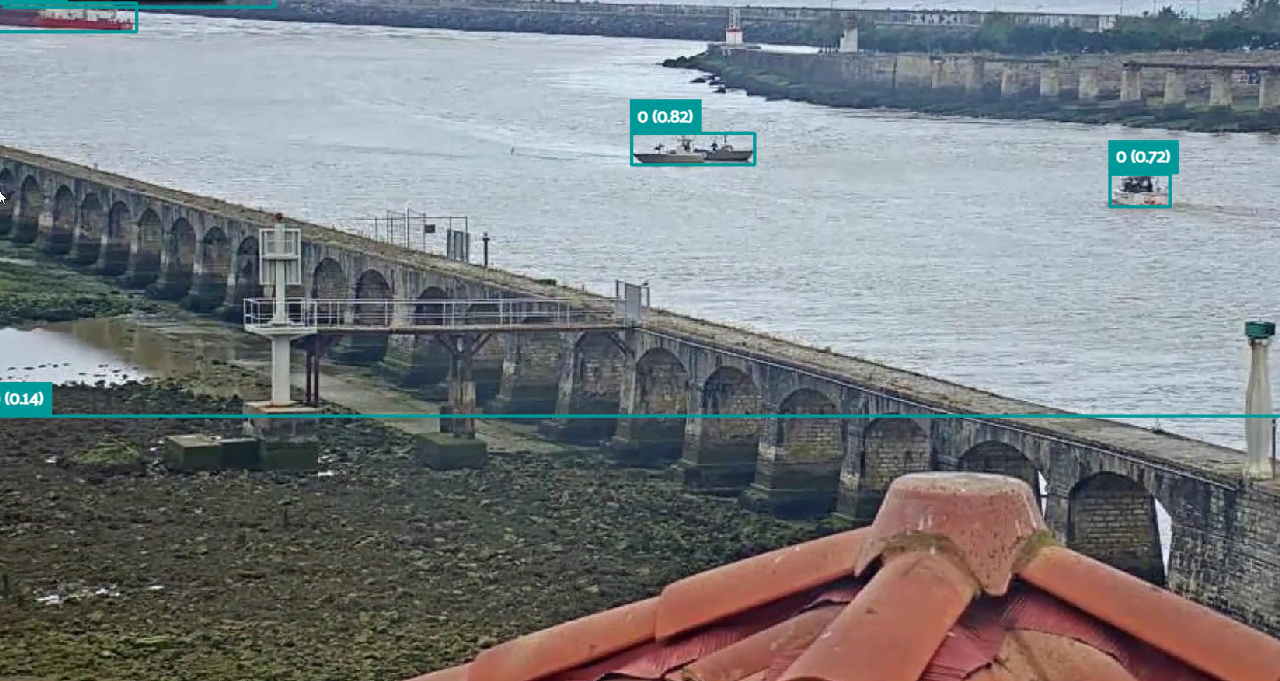
\includegraphics[width=0.5\textwidth]{./img/first_inference2.png}
    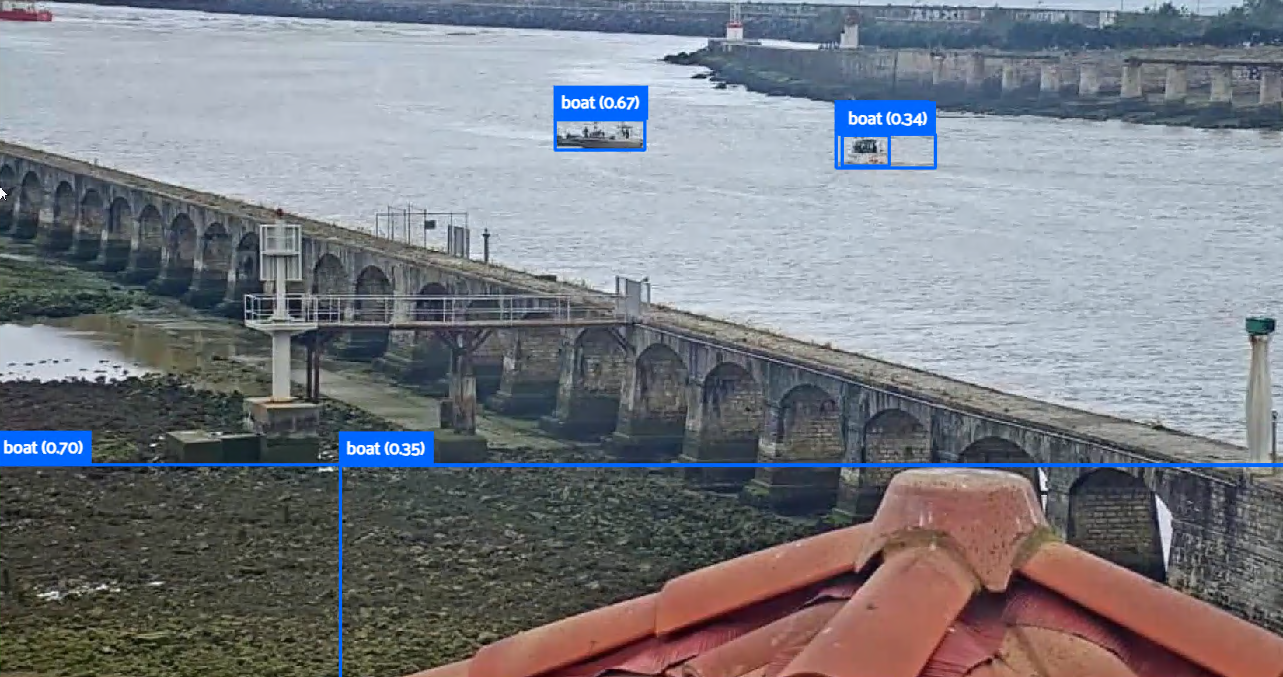
\includegraphics[width=0.5\textwidth]{./img/yolov8_inference.png}
    \caption{Comparaison entre notre premier modèle entraîné (\textit{à gauche}) et YOLOv8 (\textit{à droite}).}
\end{figure}

Après avoir analysé les images nous avons conclu que tous les réseaux, mis à part leurs scores mAP et mAR
respectifs, avaient des problèmes similaires : détection de piliers et du toit comme des bateaux.
Ceci valide encore une fois la cohérence de nos travaux par rapport à l'état de l'art.

\section{Développement du pipeline d'entraînement}

Cette section présente le fonctionnement du système que nous avons développé, de l'import des données
jusqu'à l'évaluation du modèle, en passant par l'entraînement. \\

Pour guider nos développement, nous
nous sommes renseigné sur les principes MLOps\footnote{MLOps est l'hybridation de "Machine Learning" et "DevOps".
Il s'agit d'une approche qui combine les processus de développement logiciel traditionnels avec ceux
du machine learning pour améliorer la qualité, la productivité, et la sécurité des modèles de machine learning.}.
Cette approche nous a conduit à créer un parcours stable qui permet de lancer le preprocessing\footnote{
Le préprocessing, également appelé "prétraitement" ou "préparation des données",
est un processus important dans l'analyse de données et l'apprentissage automatique.
Il consiste à mettre en forme et à nettoyer les données pour qu'elles soient utilisables
par les algorithmes de machine learning.} puis l'entraînement en quelques minutes, en
centralisant tous les paramètres.\\

En résumé, le pipelie fonctionne de la manière suivante :

\begin{enumerate}
    \item les datasets sources (prevenant de différents fournisseurs de données) sont stockés au format
    COCO ;
    \item les datasets sources sont importés dans FiftyOne, où différents traitements (comme
    l'annotation ou le filtre de similarité) peuvent leur être appliqué ;
    \item les datasets sont en suite réunis en un seul ensemble d'images appelé "input dataset" ;
    \item "input dataset" est exporté dans un dossier pour pouvoir être utilisé par YOLOX.
\end{enumerate}

Comme énoncé en section \ref{facilite_utilisation}, le pipeline doit être facile d'utilisation.
Ce sont donc deux Jupyter Notebooks qui permettent de lancer tous les scripts, le premier correspondant
au prétraitement, le second à l'entraînement. Le prétraitement contient des opérations tels que
la suppressions d'images similaires, l'agglomération de tous les datasets ou encore du clustering.
Le script d'entraînement permet de lancer l'entraînement du modèle, mais aussi l'activation du
logger\footnote{Le logger est le système permettant de monitorer les performances pendant l'entraînement.}.\\

% TODO: ajouter un diagramme de classes.

L'entièreté du pipeline est contrôlé par un fichier de configuration (\textit{voir annexe} \ref{config})
au format \texttt{json}.

Il contient les paramètres suivants pour le prétraitement : datasets à utiliser, nombre d'images pour
l'entraînement, tuilage des images, labels à conserver, différents filtres pour les images (seuil de
similarité, contraste, bruit...). Il permet aussi d'activer le calcul des embeddings\footnote{
% TODO: renvoyer vers la section qui parle des embeddings dans FiftyOne.
Les embeddings sont une représentation numériques des images.}
et régler le nombre de clusters\footnote{Un cluster est un groupe d'objets similaires ou pertinents
qui ont été identifiés et regroupés en fonction de caractéristiques communes.} pour la visualisation.\\

Pour l'entraînement, on trouve entre autres les paramètres pour le nombre d'époques, la taille de batch,
la profondeur du modèle YOLOX.\\

Concernant le monitoring de l'entraînement, nous avons d'abord utilisé Weight\&Biaises
(\url{https://wandb.ai/home}), puis Tensorboard (\url{https://www.tensorflow.org/tensorboard}). \\

Afin de conserver une trace de chaque entraînement, le pipeline permet de transferer automatiquement
les informations suivantes vers une destination pérenne : nombre d'images et de détections utilisées
ainsi que leurs sources (différents datasets), dimensions des images, classes, durée d'entraînement,
carte graphique utilisées, filtres et seuils. \\

\section{Prétraitement}

Nous présentons dans cette section l'ensemble du travail réalisé concernant le prétraitement des images
et la préparation pour les entraînements.

\subsection{Analyse des datasets}

Après avoir réunis un grand nombre d'images, nous les avons explorées pour avoir une idée de ce qu'elles
conentaient.

\subsubsection{Labels}

Pour commencer, chaque source d'image contenant des classes différentes. Les bateaux
(notre classe d'intérêt) était parfois appelée "vessel", "ship", ou encore des noms plus précis
comme "sailboat" ou "warship".\\

Pour pouvoir rassembler ces images et les utiliser, nous avons dans un premier temps
créé des dictionnaires de conversion (\textit{voir exemple en annexe }\ref{ex_dictionnaire_conversion}) de classes pour obtenir un seul label "\textbf{boat}".

\subsubsection{Similarité}
\label{similarite}

Lors de la visualisation des datasets, nous avons remarqué que plusieurs d'entre eux utilisaient les
même images. Aussi, certains étaient issus de vidéo de surveillance, ce qui produit des images
très similaires entre elles. Le risque d'avoir des images très ressemblante est le sur-apprentissage
\footnote{Le surapprentissage (ou overfitting en anglais) est un phénomène qui se produit
lorsqu'un modèle de machine learning devient trop spécifique à l'ensemble de données d'apprentissage
utilisé pour sa formation, et qu'il n'est plus capable de généraliser ses connaissances
pour prédire correctement les résultats sur des données inconnues.} ; pour éviter ce problème,
nous avons utilisé un modèle de vision (ResNet101) pour calculer les embeddings de nos images,
et créer une matrice de similarité. Ceci nous a permis d'appliquer un seuil pour régler l'hétérogénéité
de nos datasets.

\subsubsection{Exploration}

Fiftyone permet d'utiliser les embeddings pour afficher une carte (\textit{voir figure \ref{carte_similarite}})
    dans laquelle chaque point représente
une image, et la proximité des points traduit la similarité des images.
Ceci permet de sélectionner facilement des sous-ensemble d'un dataset, et rend l'exploration beaucoup
plus facile.

\begin{figure}[H]
    \centering
    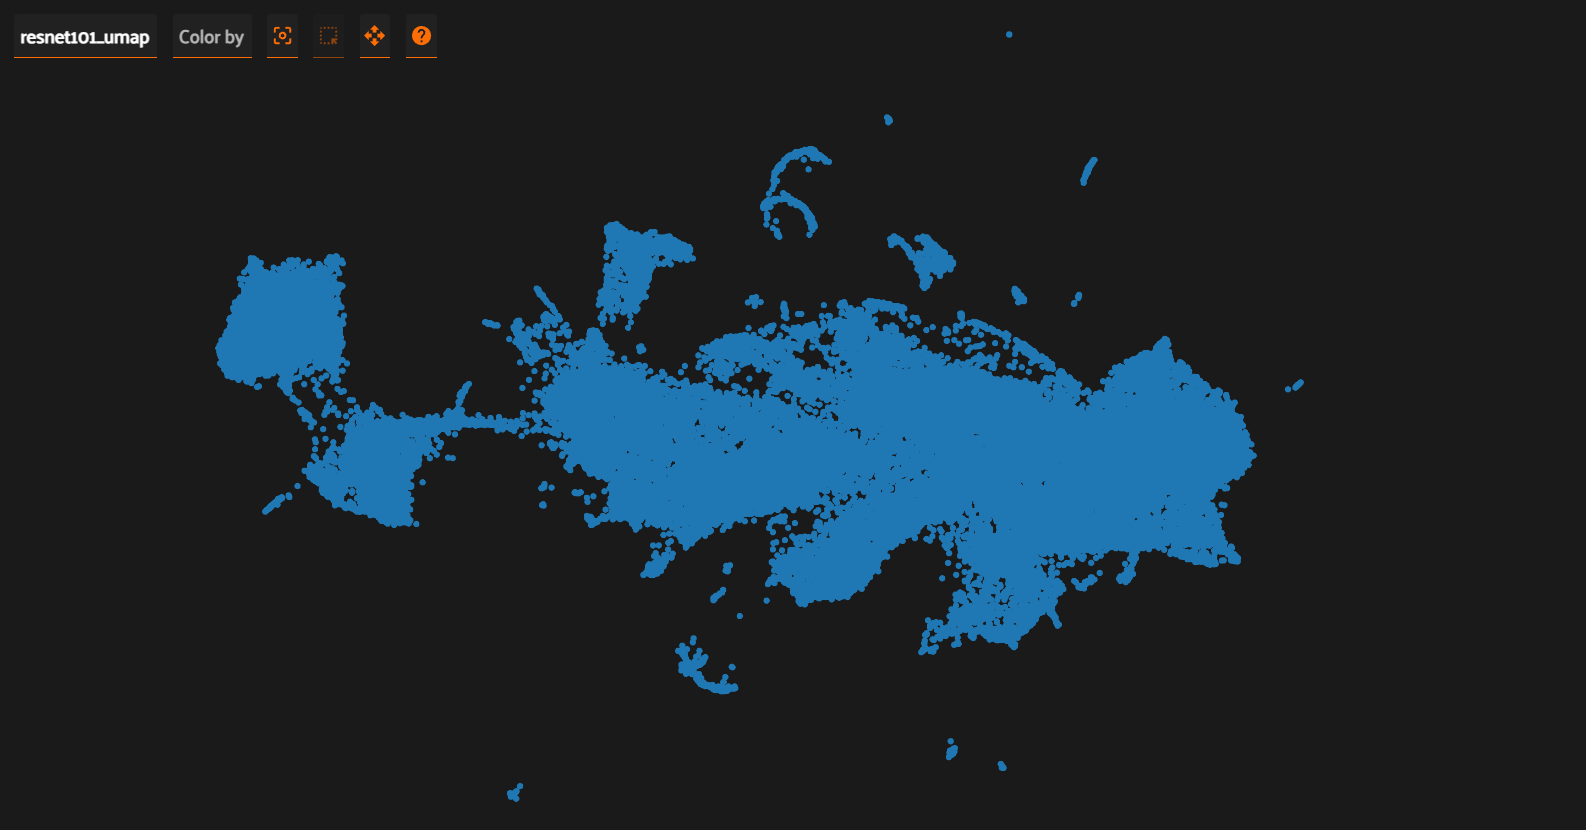
\includegraphics[width=0.7\textwidth]{resnet101_umap.png}
    \caption{Exemple de carte des embeddings dans FiftyOne}\label{carte_similarite}
\end{figure}

\begin{figure}[H]
    \centering
    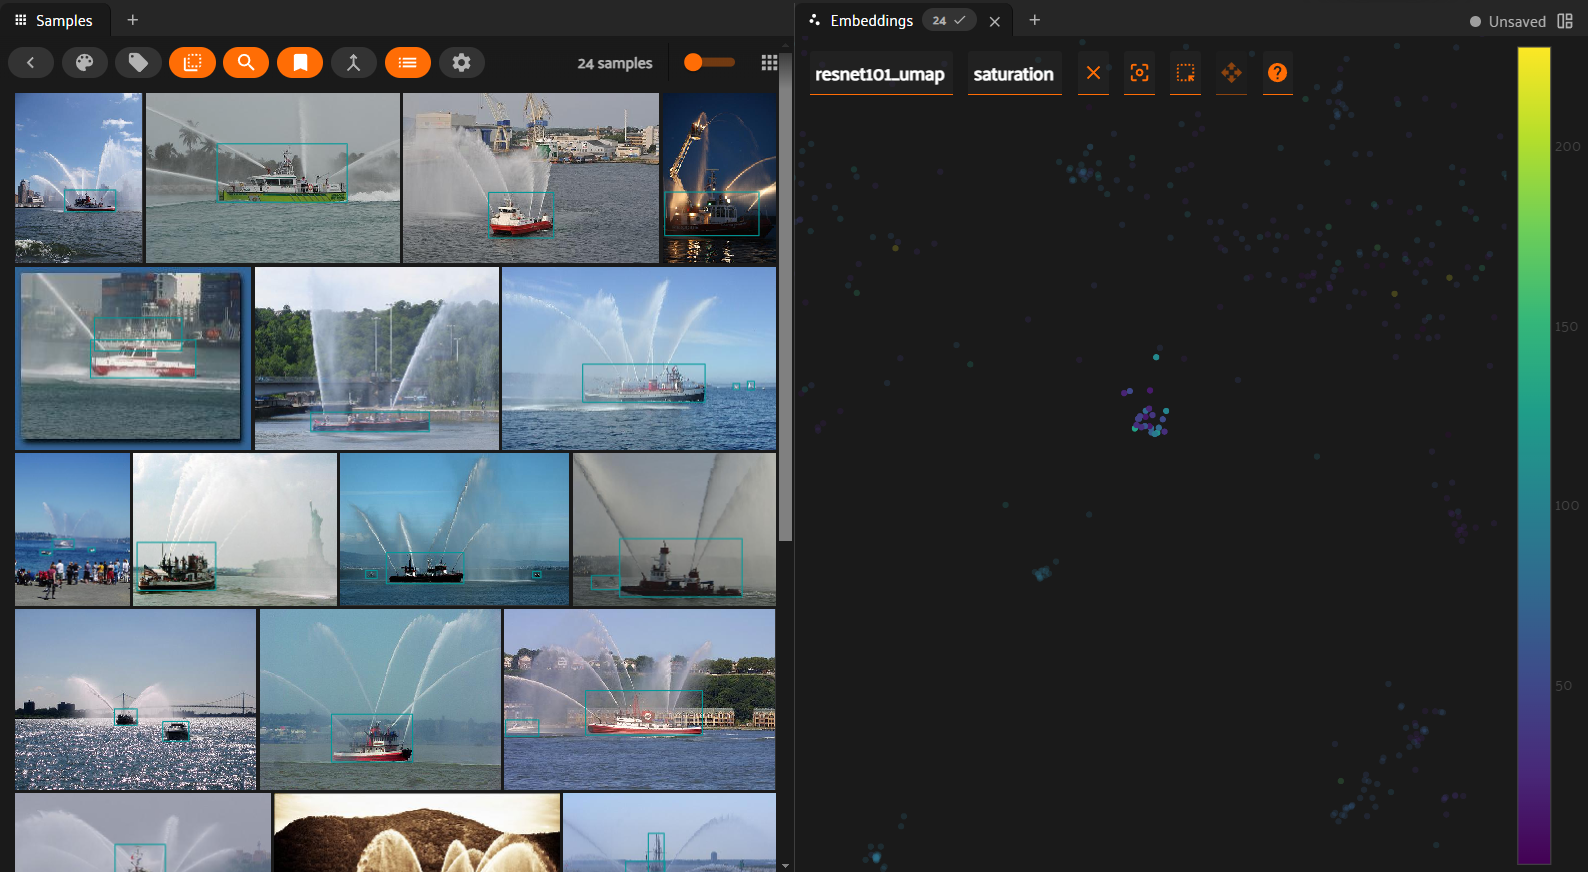
\includegraphics[width=0.7\textwidth]{bateaux_pompiers.png}
    \caption{Exemple de sélection d'un ensemble de points}
\end{figure}

Cet partie du travail nous a mené à identifier des éléments indésirables tels que des sous-marins ou
des bouées labelisées comme étant des bateaux par exemple. Nous avons aussi remarqué que certains bateaux,
selon le modèle de vision utilisé, se ressemblaient moins que d'autres : les cargos et les ferrys étaient
plus proches sur la carte que les voiliers. Cela nous a apporté une meilleure intuition.\\

Enfin, nous avons observé des erreurs d'annotation : boîte englobante décalée ou trop petite,
jouets et photos considérés comme des bateaux... Ces erreurs étant très ponctuelles et difficilement
détectables, nous avons décidé de les ignorer.\\

\subsubsection{Annotation}

Après avoir travaillé sur une seule classe de bateaux, nous nous sommes servi des outils mentionnés précédemment
pour créer nos propres annotations (\textit{voir interface de FiftyOne en annexe }\ref{clustering_interface}).
Cette action était guidée par plusieurs reflexions. La première est évidente :
prédire plusieurs classes de bateaux est un avantage indéniable du point de vue du client.
Le seconde est que, les performances variant selon les classes (certains types de bateaux sont plus faciles à
détecter que d'autres), on peut envisager d'être plus exigeant lorsque le modèle détecte une classe difficile,
c'est a dire augmenter le seuil de confiance. Cette dernière méthode pourrait permettre de réduire
le nombre de faux positifs, et donc la satisfaction des utilisateurs.\\

Comme mentionné précédemment, nous avons utilisé ResNet101 pour le calcul des embeddings,
avec cette fois une subtilité : plutôt que d'utiliser le modèle sur tout l'image, nous
l'avons utilisé uniquement sur les bateaux. En effet, deux images d'une même rivière
peuvent être considérées comme similaires, bien que les bateaux présents sur ces images
soient différents. Le calcul des embeddings sur les détections permet d'éviter ce biais.\\

Une fois les embeddings calculés et la carte de similarité crée, nous avons utilisé un algorithme
de clustering pour accélérer le regroupement des bateaux par types. Après plusieurs essais et une analyse
qualitative, nous avons choisi K-Means. Il est aussi précis que d'autres algorithmes plus complexes (DBSCAN,
OPTICS, Agglomerative...), mais surtout beaucoup plus rapide (\textit{voir documentation
de scikit-learn }\url{https://scikit-learn.org/stable/modules/clustering.html}).

\begin{figure}[H]
    \centering
    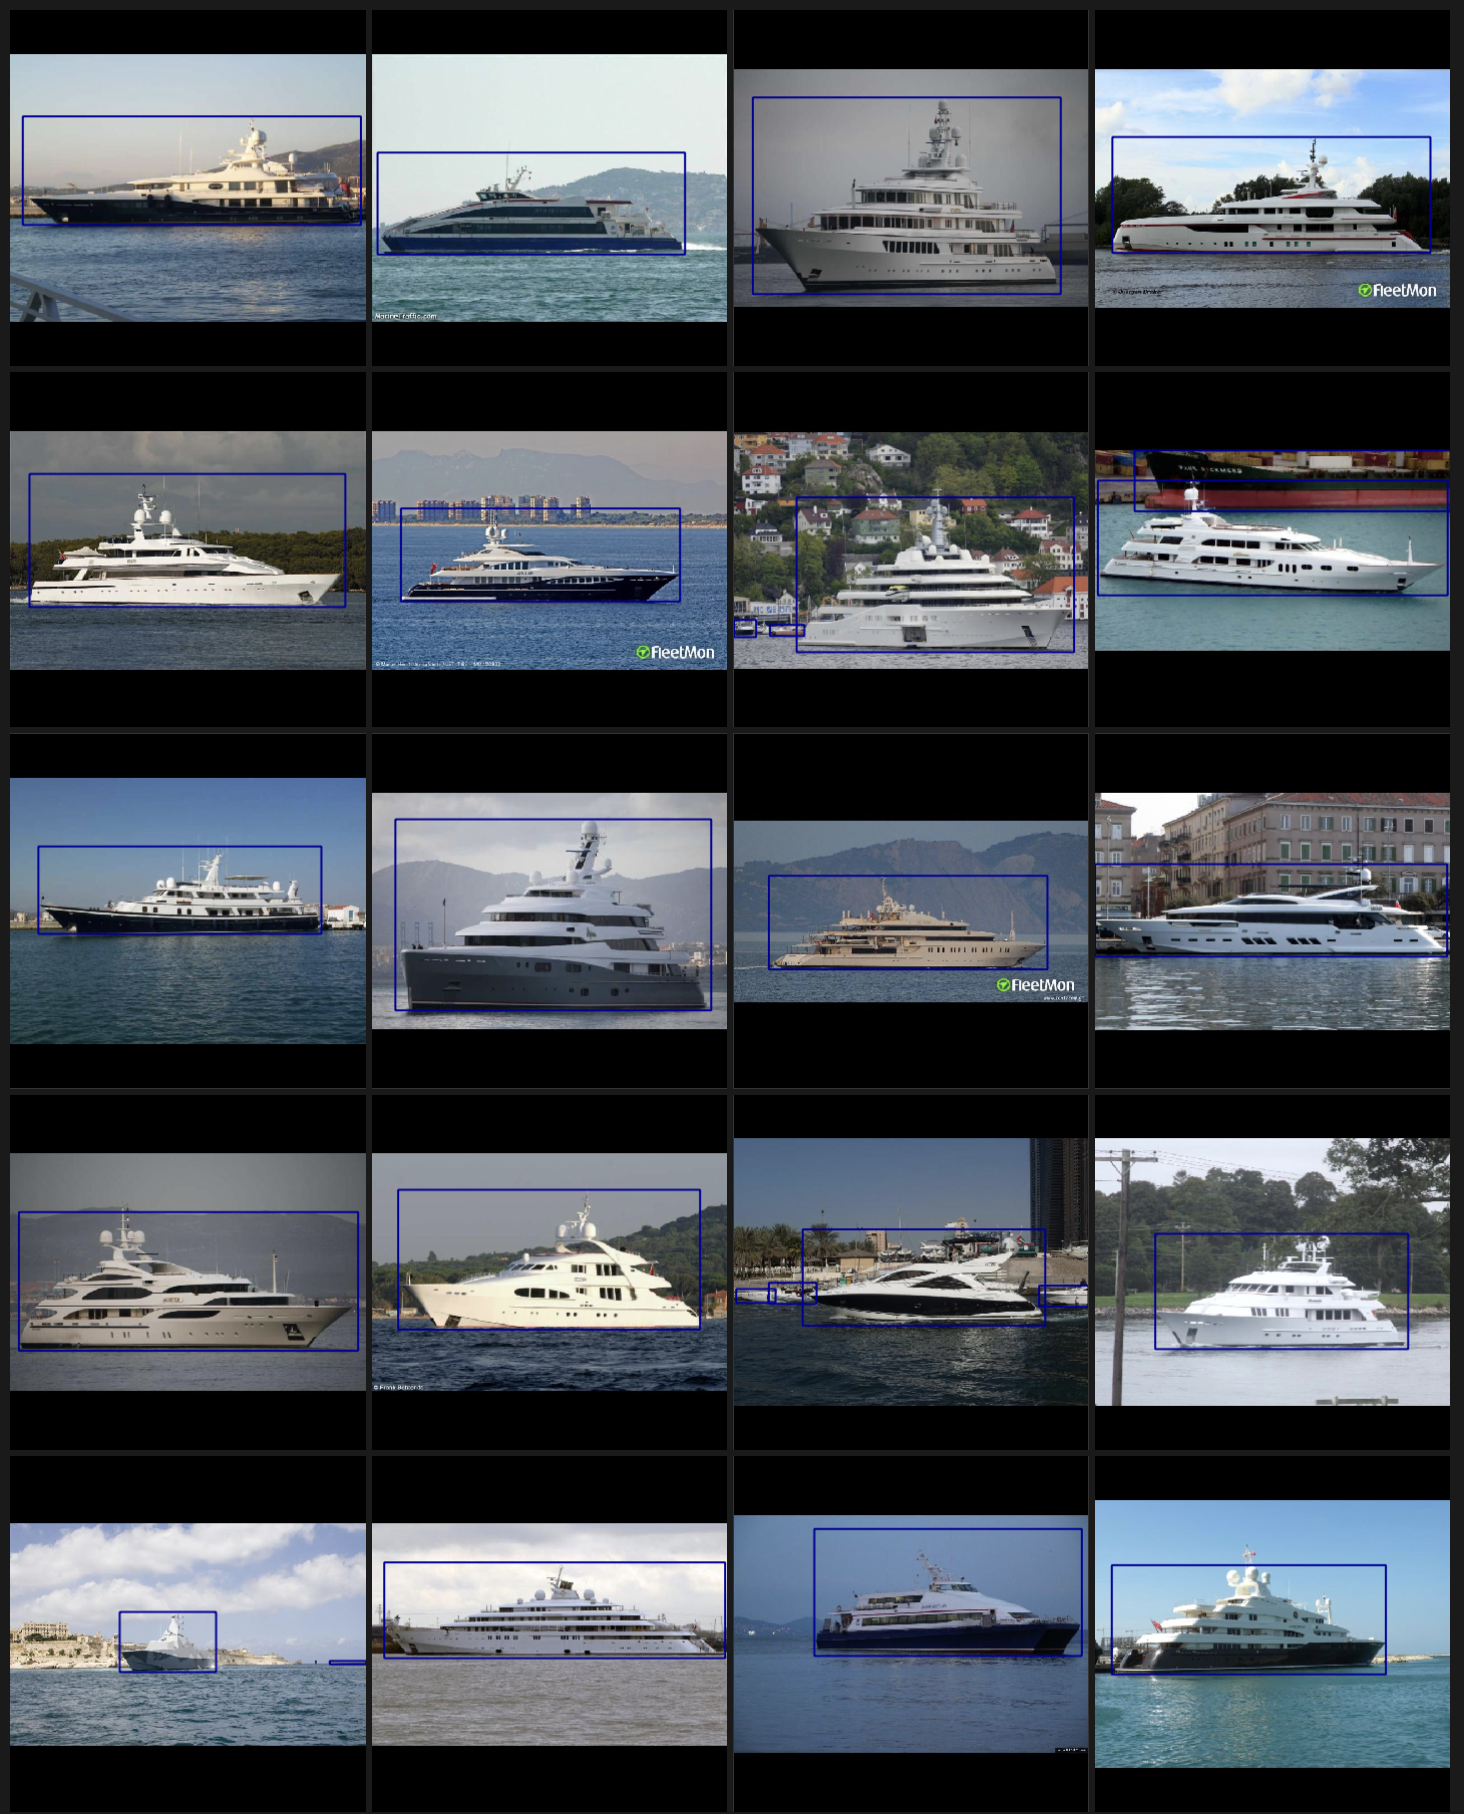
\includegraphics[width=0.3\textwidth]{./img/yachts.png}
    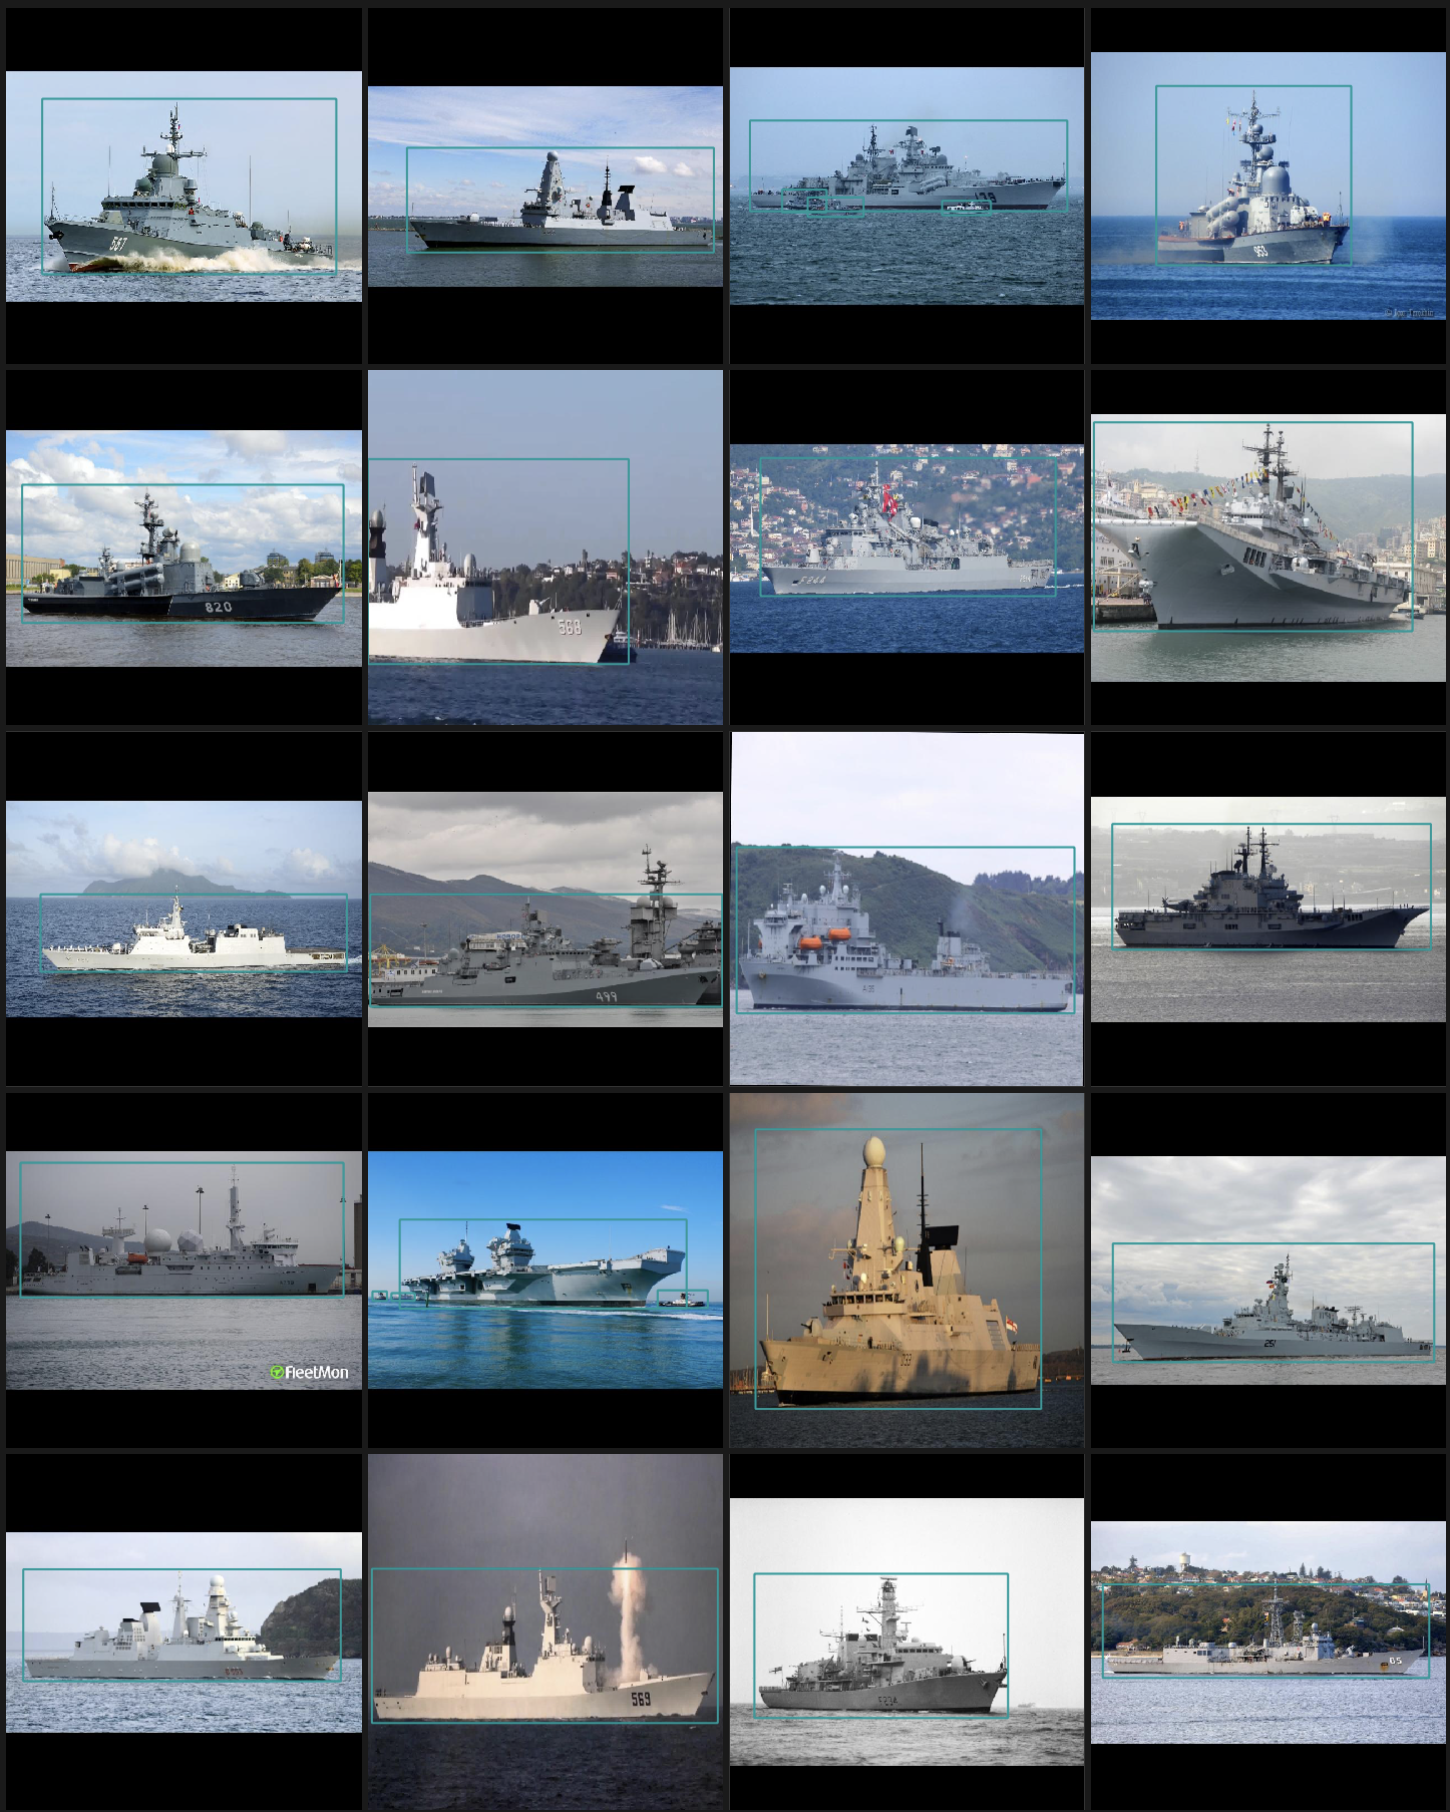
\includegraphics[width=0.3\textwidth]{./img/warships.png}
    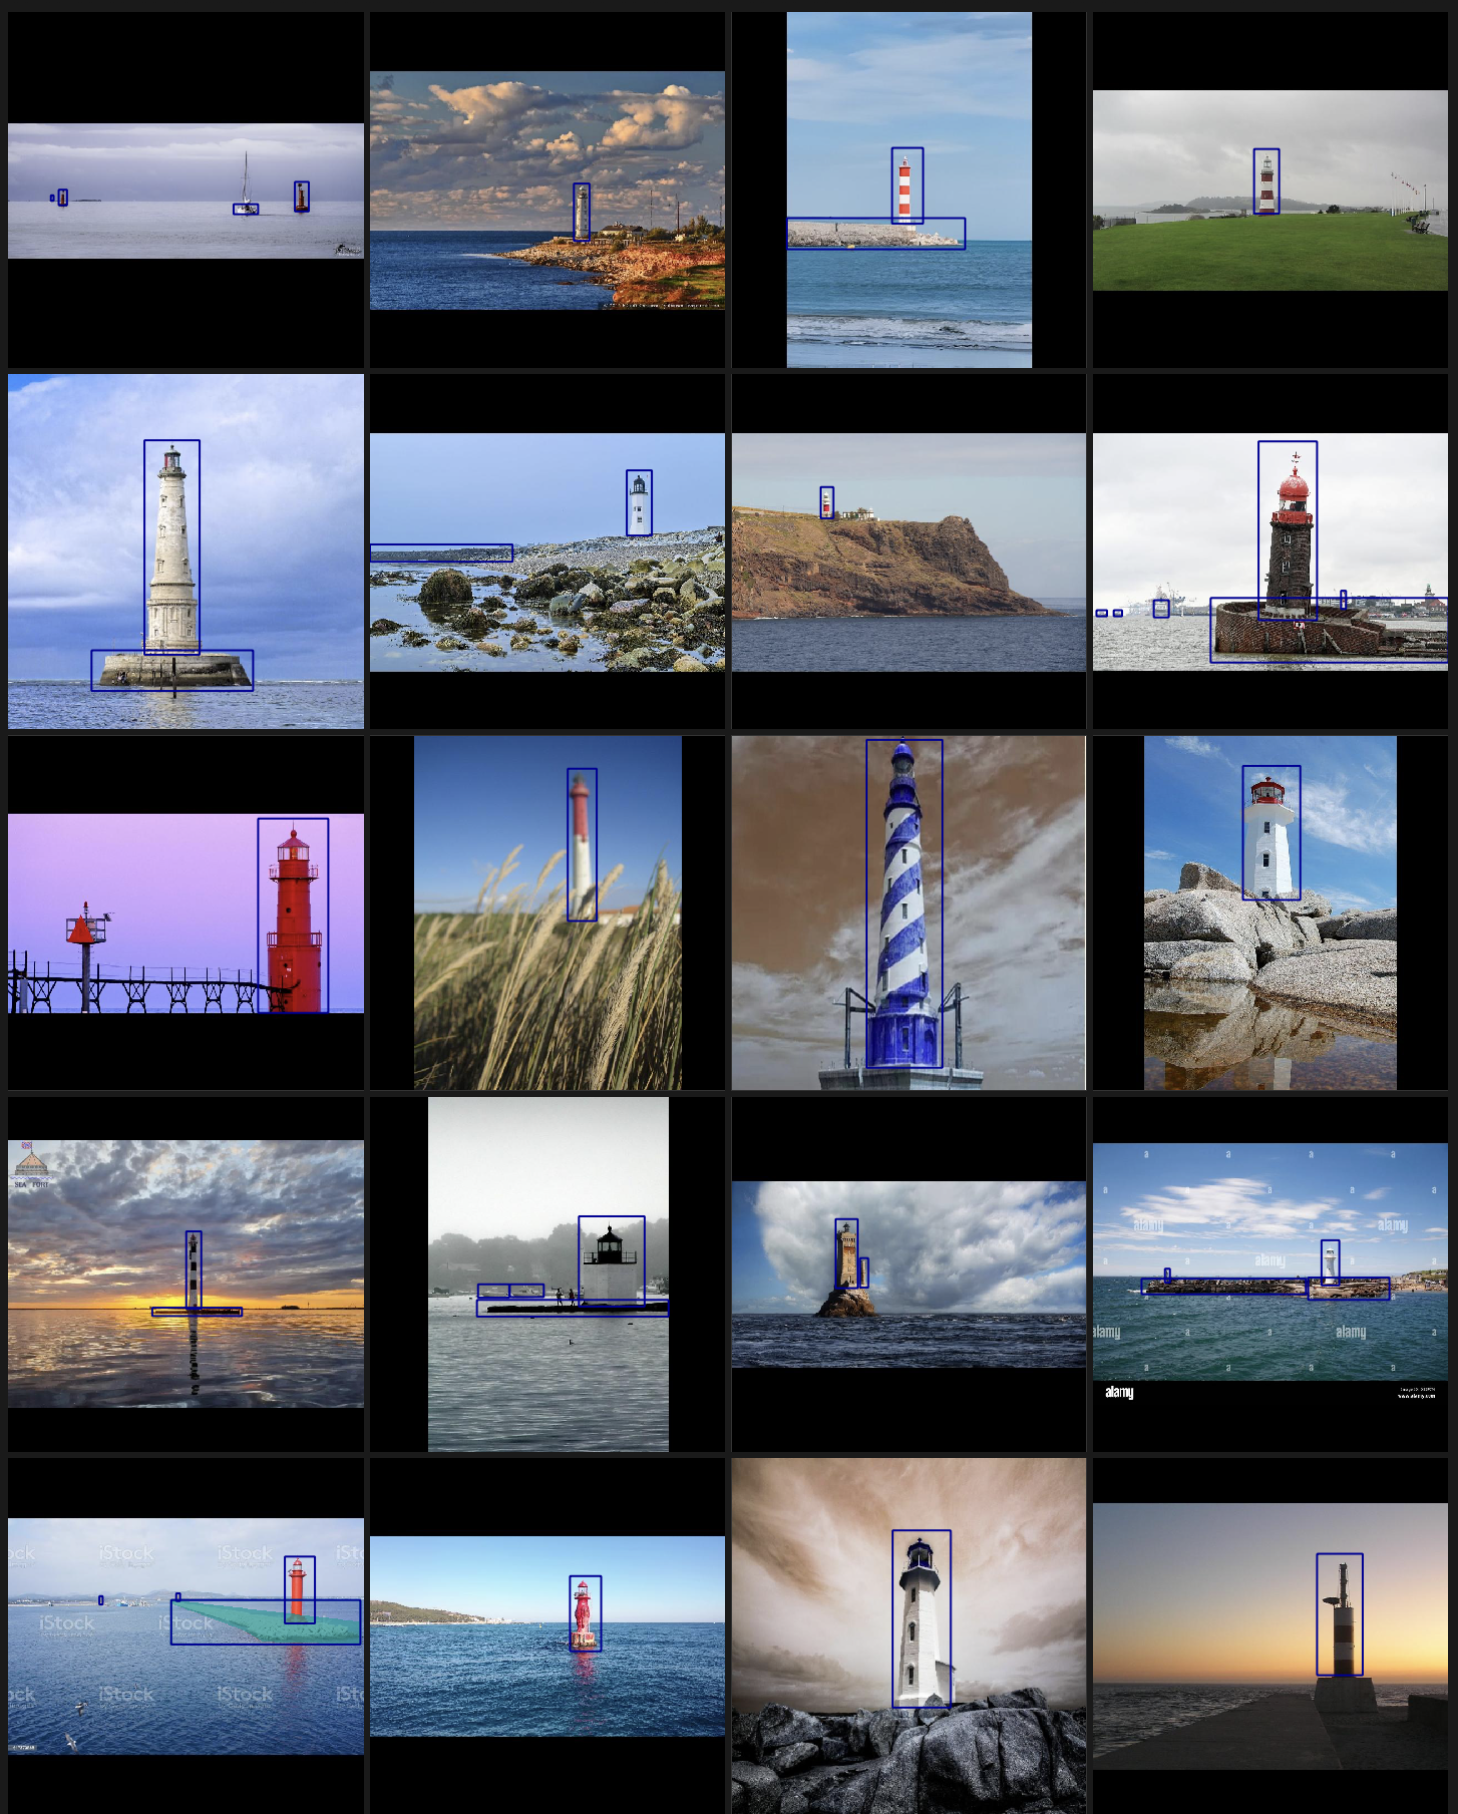
\includegraphics[width=0.3\textwidth]{./img/lighthouses.png}
    \caption{Exemples de clusters}
\end{figure}

Il faut garder à l'exprit que les exemples ci-dessus sont des cas particuliers : la plupart des
clusters contenait parfois plusieurs types de bateaux, et deux semaines de travail on été nécessaires
pour obtenir un résultat satisfaisant. En tout, 117 744 objets ont été annotés, dont 29‰ sont restés
dans la classe "\textbf{boat}" car trop difficile à classifier (en général des images floues ou trop petites).

Voici un tableau de la répartition des objets dans les différentes classes : \\


% TODO: mettre le tableau à l'horizontale.
\begin{table}[!h]
    \caption{Nombre d'objets par classes}
    \begin{center}
    \begin{tabular}{c c c c c c c c}
    \hline
    cargo & \textbf{boat} & sailboat & buoy & recreational & ferry & warship & fishing \\
    35033 & 23648 & 13153 & 9282 & 8827 & 8272 & 4593 & 3374 \\

    \hline
    cruise & lighthouse & luxury & breakwater & service & platform & bulker \\
    3172 & 2705 & 2145 & 2136 & 1080 & 273 & 51
    \end{tabular}
    \end{center}
\end{table}

Les définitions des différentes classes ont été documentées pour permettre
des annotations futures (\textit{voir annexe }\ref{classes_annotations}).
Après annotation, nous avons utilisé FiftyOne pour exporter ce dataset.

\subsubsection{Filtres}

Nous avons remarqué que la majorité des objets de nos datasets sont petits :
dans le dataset COCO par exemple, environ 41\% des objets sont petits (aire < 322),
34\% sont moyens (322 < aire < 962), et 24\% sont grand (aire > 962), selon
les définition du site de COCO.\\

Nous avons donc mis en place des filtres pour contrôler la qualité des images
utilisées pour l'entraînement. Pour cela, nous avons calculé différentes métriques
pour mesurer l'entropie, le flou, la luminosité, le contraste, l'exposition, le bruit et
la saturation.

Nous avons également mis en place un filtre qui permet d'appliquer un seuil
de similarité (calculé au préalable, \textit{voir section }\ref{similarite}).\\

Tous ces filtres sont appliqués au moment d'exporter les datasets dans le dossier
servant à l'entraînement.

\section{Entraînements}

Durant le stage, l'amélioration de l'entraînement de YOLOX pour augmenter sa précision
a nécessité plusieurs expérimentations. Au total, environ 60 entraînements ont été réalisés,
d'une durée moyenne d'environ 2 jours. \\

Chaque entraînement a donné lieu a un rapport rédigé sur OneNote et une présentation des
résultats à l'équipe. Les résultats de ces entraînements sont exposés au chapitre \ref{resultats}.

\section{Inférence}

\subsection{Conversion au format ONNX}

À la fin d'un entraînement de YOLOX, on obtient un fichier au format pth (PyTorch),
qui correspond à un dictionnaire contenant la structure et les poids du réseau de neurones.
Ce fichier doit être converti au format onnx\footnote{
Le format ONNX (Open Neural Network Exchange) est un format de fichier qui permet d'échanger
et de partager des modèles de réseaux neuronaux entre les différentes plateformes et
langages de programmation, sans perte de précision ou de performances.}
pour être utilisé pour l'inférence.\\

\subsection{Quantization}

En plus de la conversion en onnx, nous avons entrepris d'appliquer une
"quantization"\footnote{La quantization est une méthode qui transforme un modèle en une représentation
optimisée pour un certain matériel. La méthode la plus populaire est la quantization
8-bit post entraînement, car elle a un impact contenu sur la précision du modèle
et permet une accélération importante (\textit{source : }
\url{https://docs.openvino.ai/2023.3/ptq_introduction.html})}
sur nos modèles pour les rendre plus rapides lors de l'exécution.\\

Nous avons utilisé le framework OpenVINO, créé par Intel, car il permet l'optimisation pour
les processeurs de la marque, qui occupent la majorité des machines visées par les logiciels TimeZero.
La participation à une conférence d'Intel sur le sujet nous a permis de rapidement
comprendre les outils disponibles. \\

La quantization ayant un impact sur les performances, nous avons mesuré ces dernières pour
éviter une trop grande perte de précision. Selon nos tests, cette perte est d'environ 2\% maximum,
ce que nous avons jugé acceptable vis à vis du gain en performances.

Nous avons observé, sur une machine équipée d'un processeur Intel i7-8400, une augmentation d'environ
41\% en moyenne de la vitesse d'inférence : \\

\begin{table}[!h]
    \caption{Vitesse d'inférence (images par seconde)}
    \begin{center}
    \begin{tabular}{c c c}
        \hline
        Modèle & fp32 & int8 \\ \hline
        yolox\_s & 11.12 & 17.65 \\
        yolox\_s & 10.78 & 18.41 \\
        yolox\_s & 11.33 & 18.97 \\
        yolox\_s & 11.34 & 18.72 \\ \hline
    \end{tabular}
\end{center}
\end{table}

\pagebreak

\subsection{Mise en production}

Après avoir produit et optimisé des modèles, nous avons commencé, vers la fin du stage,
à discuter de l'intégration aux outils existants. Ce travail a été fait par mon maître de stage,
qui a intégré les réseaux à l'outil DebuggerTool (\textit{voir annexe \ref{debuggertool}}),
créé l'année dernière.\\

Cet outil a fait l'objet de plusieurs optimisations. La principale est que l'inférence est effectuée par tuiles,
ce qui permet de mieux détecter les petits bateaux. Aussi, il contient un tracker, ByteTrack \cite{Zhang_Sun_Jiang_Yu_Weng_Yuan_Luo_Liu_Wang_2022},
qui permet de suivre les détections.\\

Les meilleurs modèles seront prochainement sélectionnés,
et potentiellement intégrés à TimeZero Coastal Monitoring.
